\subsection*{Question 5}

Sample $p(\bm{\theta}|\mathcal{D}_1)$ using \textbf{JAGS} with the same number of iterations (after burnin) as in Q3.

\textbf{a)} Compare your results with the previous ones.

\begin{center}\rule{6cm}{0.4pt}\end{center}

Fitting a JAGS model, we now correctly estimate the growth rate of the number of cancer cells over time as we can notice on the plot below.

\begin{figure}[H]
	\centering
	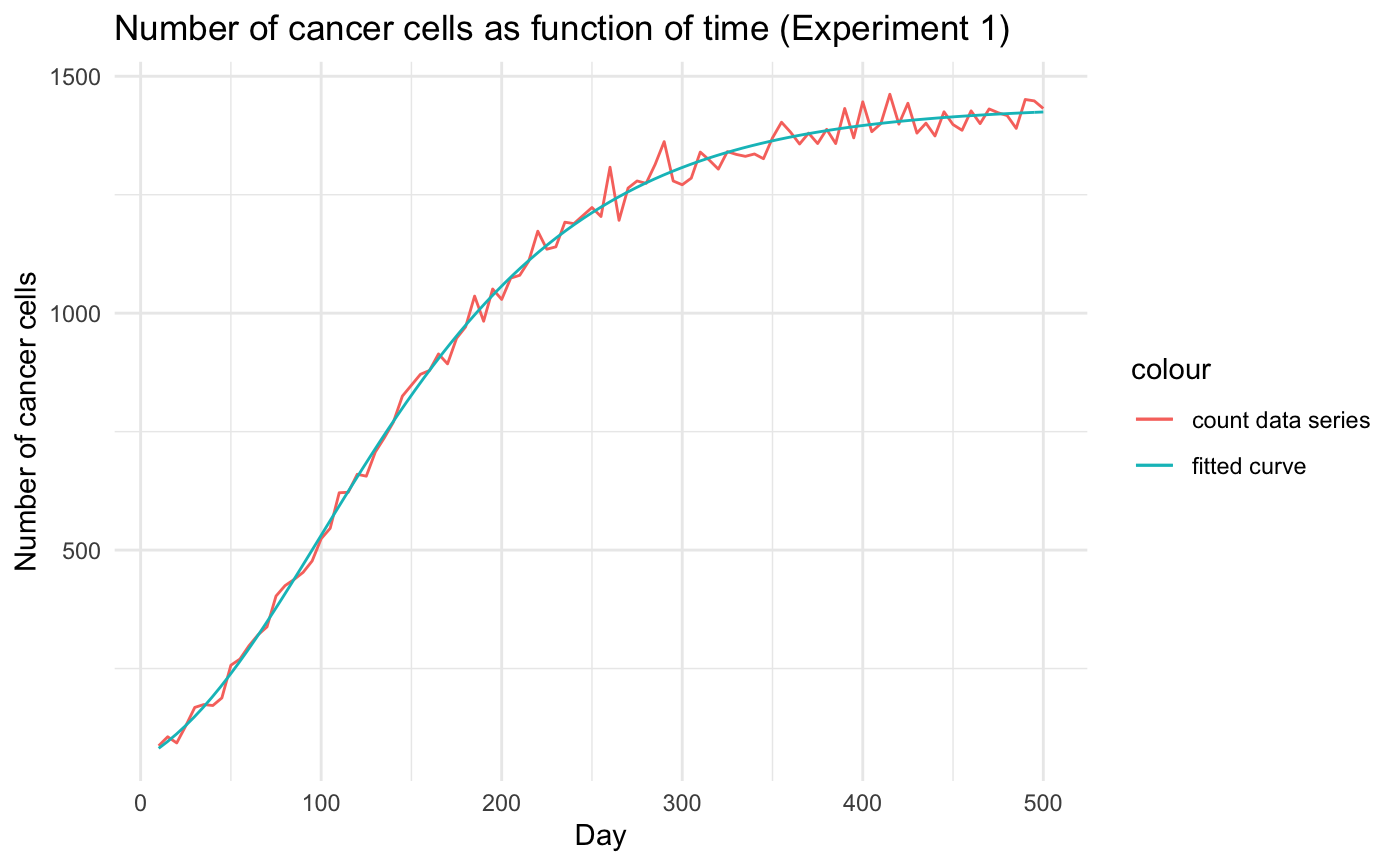
\includegraphics[width=0.7\textwidth]{figures/jags/jags_fitted_curve.png}
	\caption{Comparison of the observed count data series for experiment 1 (\textit{black}) with the fitted curve for $\mu(t)$ (\textit{red})}
	\label{fig:jags-fitted-curve}
\end{figure}

\textbf{b)} Sample the predictive distribution of the number of cells at time $t = +\infty$ and report a point estimates and a credible interval for that quantity.

\begin{center}\rule{6cm}{0.4pt}\end{center}

